% 1. in union-find subsection make function names in text a different
%    font
% 2. include parameters of size-constrained add-edge on randomized graph
%    in table
% 3. more analysis of SC AE results
%#######################################################################

We introduce several algorithms for generating brain parcellations. The
algorithms in this chapter are all local search heuristics; they begin
with $n$ unconnected vertices and iteratively join adjacent ones into
components until some stopping criterion is met.

For each algorithm, the resulting parcellation is presented, discussed,
and evaluated according to the criteria introduced in the previous
chapter.

\section{Unconstrained Add-Edge}

The first and simplest algorithm starts with an empty graph of $n$
vertices and sequentially adds edges between adjacent voxels in order of
highest sample distance correlation, until the graph has some
prespecified number of connected components $k$.

We will refer to this algorithm as ``Unconstrained Add-Edge''. A naive
implementation of would re-compute the number of connected components in
the graph (using linear-time bread-first or depth-first search) after
each addition of an edge, resulting in a costly $O(EN)$ time complexity.
A more efficient implementation takes advantage of the fact that each
addition of an edge decreases the number of components in the graph by
at most 1. Hence the algorithm needs only to compute the number of
connected components after adding $c - k$ edges, where $c$ is the
current number of connected components of the graph, beginning at $n$.

Another implementation uses a binary search-type strategy and is
$O((n + E) \log E)$. The idea is to ``search'' for the last edge to add
to the graph by maintaining a range of possible last edges. In each
iteration, the algorithm would add to the graph edges 1 to the midpoint
of this range, compute the number of connected components, and adjust
the range based on whether the number of components is higher or lower
than the target $K$.

The Unconstrained Add-Edge algorithm produces severely imbalanced
parcellations. In the 100-component graph, there was one component
containing over 99.9\% of all the vertices in the graph. This leads
to a modification that prevents some edges from being added when a
size constraint is violated.

\section{Size-Constrained Add-Edge}

The Size-Constrained Add-Edge algorithm works in a similar manner to the
unconstrained version, adding edges to the graph in decreasing order of
distance correlation. The Size-Constrained version differs by applying
a filter to each edge considered, adding the edge only if at least one
of the two following conditions are met:

\begin{enumerate}[1.]
\item
At least one of the two components bridge by the edge is of size less
than some prespecified parameter $s_{\min}$.

\item
The union of the two components is of size $\leq s_{\max}$.
\end{enumerate}

The restriction on adding new edges was not successful in creating
balanced partitions. For sake of completeness, we documented our
implementation.

The naive implementation must use BFS/DFS in each iteration to compute
the sizes of the two components to be connected by an edge, and hence
must have time complexity $O(EN)$. Fortunately, there is a way to
sublinearly update information on the components of the graph, using
the union-find data structure.

\subsection{Union-Find}

The core Union-Find data structure begins with an empty graph of $N$
vertices and supports two operations. union(i, j) adds an edge between
vertices $i$ and $j$. root(i) returns an identifier for the component
to which vertex $i$ belongs. All vertices in the same component have the
same root. We modified Union-Find to support an additional operation.
component\_size(i) returns the number of vertices belonging to the
component containing $i$.

Union-Find represents each component as a rooted tree, with vertices in
the graph mapping to nodes in the tree. Information about the tree is
stored in two arrays of length $N$, parent and size, which are subject
to the following invariants.

\begin{enumerate}[1.]
\item
For each node i, parent[i] = node i's parent on the tree, unless i is a
root node. If i is a root node, then parent[i] = i.

\item
Nodes i and j are in the same component if and only if they are in the
same tree, if and only if they share the same root node.

\item
If i is a root node, then size[i] = the size of the component, or the
number of nodes in the tree. If i is not a root node, then size[i] can
be anything.
\end{enumerate}

A baseline implementation of the three functions is

\begin{algorithm}
\caption{Union-Find}
\begin{algorithmic}

\Function{root}{i}
    \While{parent[i] $\neq$ i}
        \State i $\gets$ parent[i]
    \EndWhile
    \State \Return i
\EndFunction
\State 

\Function{union}{i, j}
    \State parent[root(j)] $\gets$ root(i)
\EndFunction
\State 

\Function{component\_size}{i}
    \State \Return size[root(i)]
\EndFunction

\end{algorithmic}
\end{algorithm}

In addition to the baseline code above, there are two important
optimizations:

\begin{enumerate}[1.]
\item
Weighted union maintains information of the sizes of each component so
that the root of the smaller component always becomes a child of the
larger component's root.

\item
Path compression flattens the tree with each call to root. Specifically,
when root is called on node $i$, each node traversed from $i$ to the
root has its parent set to be the root.
\end{enumerate}

With these two optimizations, the time complexity of root, union, and
component\_size has been shown to be at least as good as $O(\log^* N)$
where $\log^*$ is the iterated logarithm, defined as the number of
times the natural log must be applied to $N$ so that it becomes less
than or equal to 1.

\section{The Contractible Graph Data Structure and
Edge-Contraction Algorithm}

We propose a new data structure called the \textit{Contractible Graph}
(CG) for brain parcellation. The rationale behind the CG is a heuristic
procedure for partitioning a graph into somewhat balanced components
so as to minimize the Boundary-Score (\ref{boundary-score}) or maximize
the Adjacency-Score (\ref{adjacency-score}).

The CG is a mapping of the vertices of the original graph to the
vertices of a new graph. The vertices of the CG are called
\textit{components} and between any two components there exists exactly
one weighted edge, henceforth called a \textit{link}. The weight
of a link $w(A,B)$ between two components $A$ and $B$ in the CG equals
the average weight of all edges in the original graph between vertices
mapped to $A$ and vertices mapped to $B$. If no such edges exist,
the weight of the link is $0$. Formally,

\[ E(A,B) = \{(i, j) \in E : i \in A, j \in B\} \]
\[ w(A,B) = \begin{cases}
    \frac{1}{|E(A,B)|} \sum_{(i,j) \in E(A,B)} w_{ij} &
        \text{if } |E(A,B)| > 0 \\
    0 & \text{otherwise}
\end{cases} \]

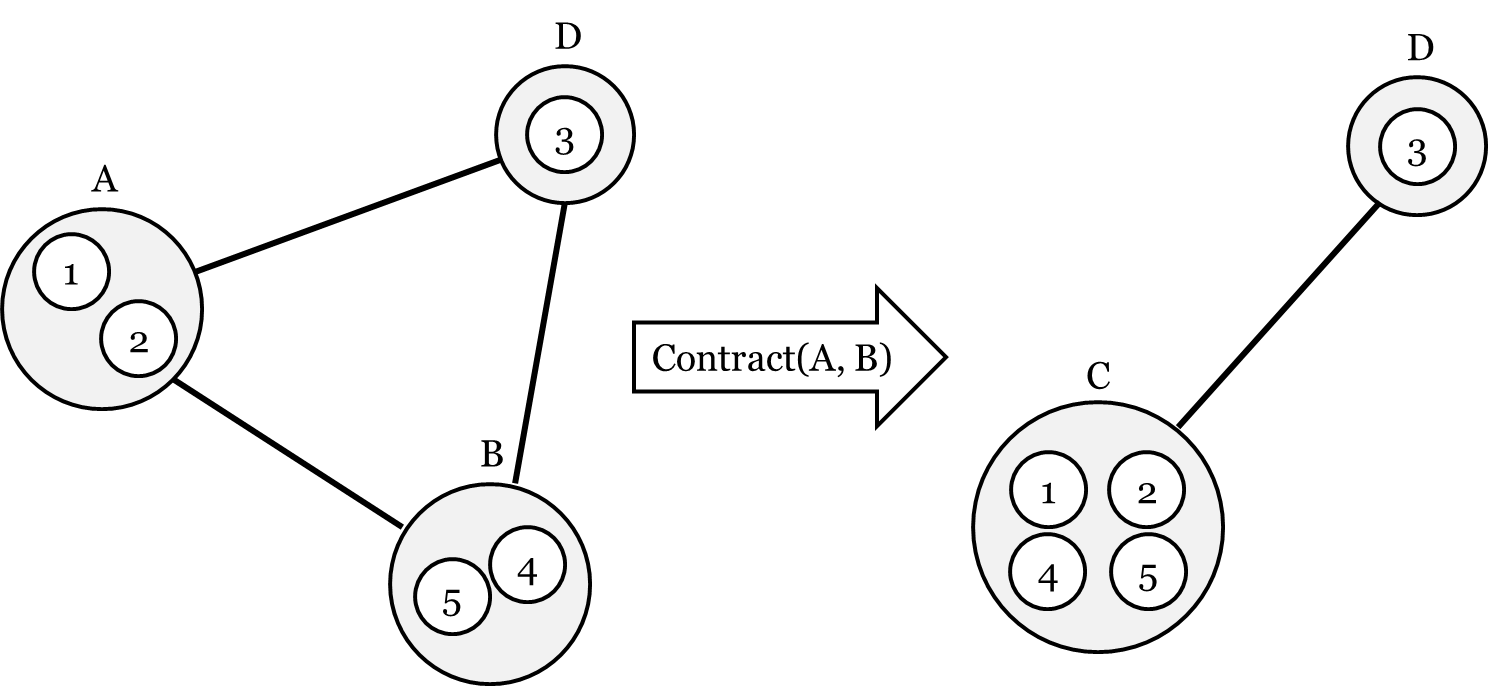
\includegraphics[scale = 0.5]{4_contractible_graph}

The \textit{size} of a component is the number of vertices it contains.
A \textit{contraction} of a link $(A,B)$ in a CG replaces components
$A$ and $B$ with a new component (call it $C$) containing all vertices
mapped to $A$ or $B$, as illustrated in the figure above.
Component $C$ has one link to every other component in the CG, whose
weights are the mean of the weights of the corresponding vertex edges,
or $0$ if no edge exists. Thus the contraction operation maintains the
link-invariant property of CG. This leads to the Edge-Contraction
algorithm, which begins with the original graph with all vertices as
singleton components and contracts edges in a certain order until the
graph has only $k$ components in all.

\begin{algorithm}
\caption{Edge-Contraction}
\begin{algorithmic}
\State \textbf{Input:} Undirected positive-weighted graph $G$ and
       target component number $k$
\State Create a CG from $G$ so that every vertex maps to
       a unique component
\Repeat
\State $\mathcal{S} \gets$ smallest component(s) in the CG
\State $(A,B) \gets \argmax{A \in \mathcal{S}} w(A,B)$
\State Contract $(A,B)$
\Until{CG has $k$ components}
\State \textbf{Output:} Components of CG
\end{algorithmic}
\end{algorithm}

Why does Edge-Contraction work better than the previous algorithms?
The Edge-Contraction algorithm attempts to address two problems of
the Size-Constrained Add-Edge algorithm: poor Adjacent-Score relative
to randomized graph and unbalanced parcels. We hypothesized that one
reason for a relatively low Adjacent-Score might be the following
scenario: when a vertex is added to a component, it might have multiple
edges to that component. One edge might have a very high weight; this is
the one that is officially ``added''. However, the other edges with far
lower weights are implicitly added as well, lowering the average edge
weights within the component.

The Edge-Contraction algorithm handles this issue by maintaining that
there can be at most one edge between any two components A and B, and
further that the weight on such an edge is the mean of the weights on
all edges that connect a vertex in A with a vertex in B.

\subsection{Implementation using Multi-Edge Adjacency List and
Priority Queue}

The adjacency list is the most common implementation choice for sparse
graphs and it lists, for each node in the graph, the nodes connected to
it by an edge and the weight of that edge.

In a Contractible Graph, the weight of the link between two components
$A$ and $B$ depends on all edges between vertices in $A$ and vertices in
$B$. Therefore our implementation of the CG data structure uses an
extended variant of the adjacency list that allows for multiple edges
between two nodes.

The Multi-Edge Adjacency List associates every \textit{pair} of
components connected by a non-zero link to the set of edges that
comprise that link. In \textbf{R}, this is achieved by a list of lists.

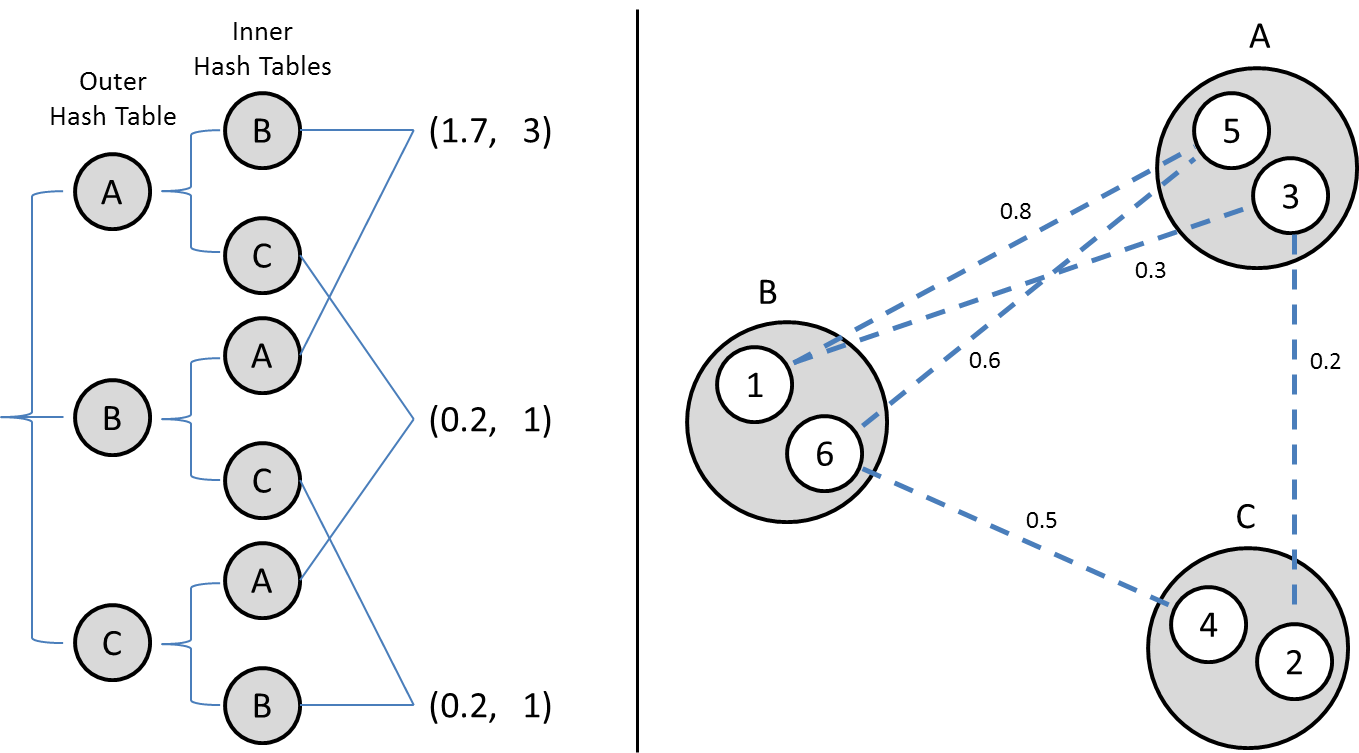
\includegraphics[scale = 0.5]{4_cg_implement}

Implementing the contraction of components $B$ and $C$ into a new
component $D$ on this list of lists requires the following steps:

\begin{enumerate}
\item
Compute $\mathcal{X}$, the set of all components that either $B$ or $C$
is linked to.

\item
Create a new element in the outer list, $D$, and associate it with an
empty inner list.

\item
For each component $X \in \mathcal{X}$,
\begin{itemize}
\item
Find $w(X)$, the weights of the set of all edges connecting $X$ to $B$
and $X$ to $C$.

\item
Delete elements $B$ and $C$ from the inner list of $X$.
Add a new element $D$ and map it to $w(X)$.

\item
In the inner list of $D$, add a new element $X$ and map it to $w(X)$.
\end{itemize}

\item
Delete $B$ and $C$ from the outer list.
\end{enumerate}

Incidentally, we note that it is also possible to implement the average
edge property of the CG without the Multi-Edge Adjacency List, by
recording for each pair of components, the \textit{sum} of edge weights
and the number of edges rather than a set of all original edge weights.
This allows for a more space and time efficient implementation, but this
simplification was unfortunately overlooked in the first implementation
of Edge-Contract.

Having described the contraction step, we will next discuss how to
efficiently locate the link to be contracted.
In computer science, a \textit{Priority Queue} data type is a set of
ordered (in the sense that for any two objects one has greater or equal
priority to the other) objects that supports the following operations:

\begin{itemize}
\item
\textit{add(obj)}: Adds an object to the set.

\item
\textit{remove\_minimum()}: Removes and returns an object with the
smallest priority in the set.
\end{itemize}

Using the heap data structure, the above two operations both run in
$O(\log n)$ time.

Each component on the CG will be associated with an element of the
priority queue. The priority of component $A$ is defined as
\[ |A| - \max\;w(A) \]
where $w(A)$ is the set of weights of links between $A$ and any other
component. Since our graph edge weights are all between 0 and 1,
the smallest priority element in the queue is the first to undergo
contraction in our algorithm, provided the max link weight is up-to-date.

If components $A$ and $B$ are contracted, and there is a component $C$
with positive links to both $A$ and $B$, then the $C-A$ and $C-B$ links
will be replaced by a $C-(AB)$ link with a different weight. If either
$C-A$ or $C-B$ links happened to be the maximum-weighted links of $C$,
then $C$'s position on the priority queue may no longer be accurate, and
its true position may be further down the queue.

To address this issue, the max weight link of the minimum priority
component must be re-computed when the element is removed from the queue.
If the component's actual priority is not the minimum, then it is
re-inserted into the queue with updated priority.
Additionally, the minimum priority component may no longer exist in the
CG due to contraction with another component. In this case it is simply
discarded.

Without using an efficient priority queue, the linear searching method
of finding the next link to contract results in a $O\big(n (n-k)\big)$
time algorithm. Using the priority queue the time complexity of
Edge-Contraction is $O \big((n - k) (m + \log n)\big)$, where $m$ is
the average number of positive links a component has.

\subsection{Results and Optimal Number of Components}

\begin{figure}
\caption{Results of Edge-Contract for Different Component Numbers}
\csvautotabular{4_edge_contract_results.csv}
\end{figure}

The Edge-Contraction algorithm has the benefit of requiring only one
parameter, the target component number. 